%!TEX root = ../thesis.tex
%*******************************************************************************
%*********************************** First Chapter *****************************
%*******************************************************************************

\chapter{Introduction}  %Title of the First Chapter

\graphicspath{Chapters/Chapter1/Figs/}



%******************************* %First Section  *****************************
\section{The honeybee and the division of labor} %%TODO: title good?

A honeybee (\textit{Apis mellifera}) colony manifests multiple fascinating
examples of complex adaptive behaviour. Localized cues exchanged between
individuals amount to emergent directional signals for the entire colony in ways
heavily investigated, but often still not completely understood. 

One of the most notable and well-researched adaptive mechanisms of a colony is
its division of labor (DOL). During the winter (a season of low activity for the
bees), the colony focuses on survival and its workers are generalists,
performing sets of tasks not easily distinguishable from those of other workers.


For the spring-summer season, however, the hive’s goals change and along with
them, the patterns of labor division. Hive growth and resource accumulation take
priority, and specialization eventuates amongst workers. They begin to fill
distinct roles, the allocation of which highly correlates with age (an effect
known as temporal polyethism) - but is also grounded in the colony’s current
needs and in environmental factors affecting it (adaptive behaviour)
\citep{seeley_adaptive_1982}. Groups of workers that can be categorized as
performing the same set of tasks are commonly referred to as castes. It is
common to recognize four of them in the temporal caste system that the worker
bees exhibit in the summer \citep{johnson_division_2010}: 
\textit{cell cleaners, nurses, middle-aged bees(MABs),} and \textit{foragers}. 
This work concentrates on the transition between
\textit{MABs} and \textit{foragers}, possibly the most distinguishable and
important in the lifecycle of a bee.


%******************************* %Second Section  *****************************
\section{The foraging phase}
The foraging phase is the last one in a bee’s life and comes with an increased
risk of death. It is often proposed that this has to do with the extreme strain
foraging puts on their bodies - essentially causing them to work themselves to
death. This is supported for example by \citep{williams_age_2008},
where honeybee flight was shown to cause extremely high metabolic
rates and induce oxidative stress, likely significantly accelerating the ageing
process and causing early deaths. On the other hand, the results of
\citep{visscher_survivorship_1997} suggest that foragers’ deaths are usually
caused not by senescence, but rather by the heightened risks of outside life
that come with their function (such as the risk of predation). According to
their findings, forager mortality rates are constant with respect to age (and
not accelerating, as would have been suggested by the body strain hypothesis). 

Regardless of the reasons behind it, foraging nearly always ends in the death of
the bee. That fact, combined other basic metrics of the foraging phas should allow 
us to get a very simple estimate of the foraging period, which we could then use for
basic validation of the results we produce with our methods.

% Please add the following required packages to your document preamble:
% \usepackage{booktabs}
\begin{table}[h]
\centering
\caption{Basic metrics for foraging phase lenght and forager survivorship, according to \cite{visscher_survivorship_1997}}
\begin{tabular}{|l|c|}
\hline
\multicolumn{1}{|c|}{\textit{Metric}}                    & \textit{Value}\\ \hline
Mean lifespan of foragers (+ 1 standard error)  & 7.7days ± (0.75 days) \\ \hline
Range of values for a forager lifespa           & 2 -17 days            \\ \hline
Probability of death per hours of foraging      & 0.036                 \\ \hline
Probability of death per day of being a forager & 0.161                 \\ \hline
Probability of death per trip                   & 0.023                 \\ \hline
\end{tabular}
\end{table}

%******************************* %Third Section  *****************************
\section{The \textit{BeesBook} project}
This work operates on data from the 2016 iteration of the BeesBook project
\citep{wario_automatic_2015}. A hard- and software framework was set up, allowing
for high-confidence tracking of all individuals over the entire lifespan of a
honeybee colony. It is the first dataset ever collected (to our knowledge) that
is extensive enough to provide a comprehensive view of a hive’s life,
maintaining the spatial, temporal and social context of the information it
stores. 

\begin{figure}[htbp!] 
\centering    
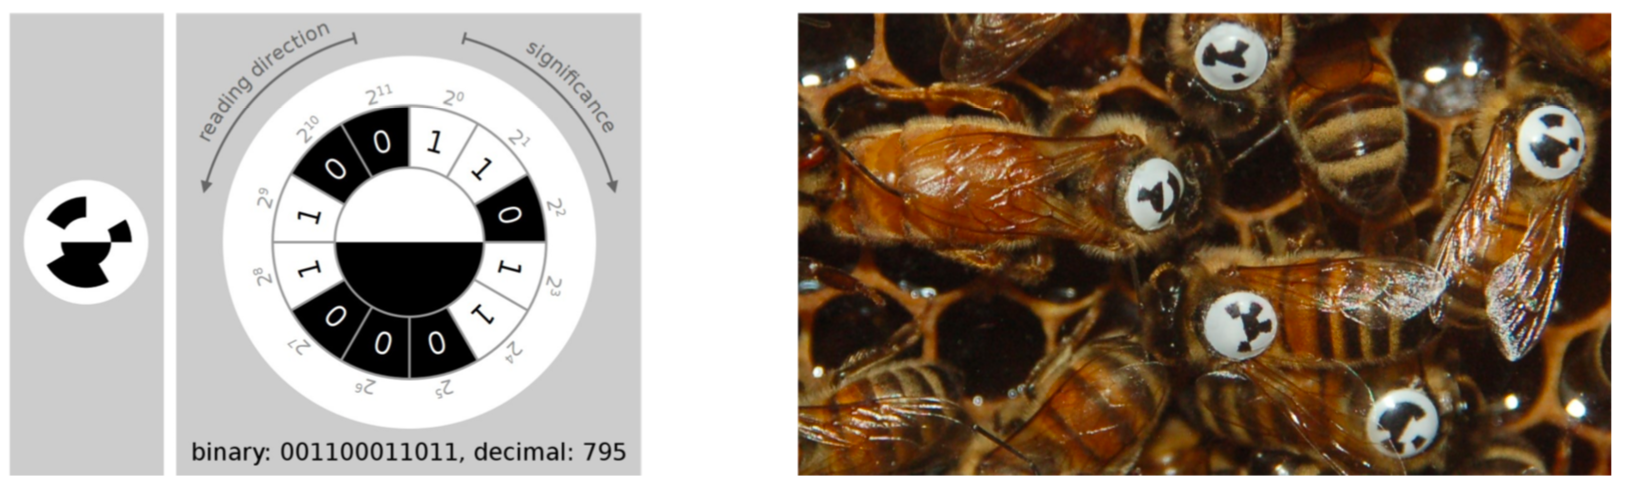
\includegraphics[width=1.0\textwidth]{Chapters/Chapter1/Figs/tag-design-boenisch.png}
\caption[tag-design-boenisch]{The tag used for marking individuals in the BeesBook project uses 12 binary-encoding segments arranged around two semi-circles (that are used to determine orientation of the tag before decoding it). The tag is glued onto the thorax such that the white semi-circle is rotated towards the bee’s head. The tags are designed to endure all activities, including cell inspections and foraging trips. 
\\(Figure adapted from \cite{boenisch_tracking_2018})}
\label{fig:tag-design-boenisch}
\end{figure}


\begin{figure}[htbp!] 
\centering    
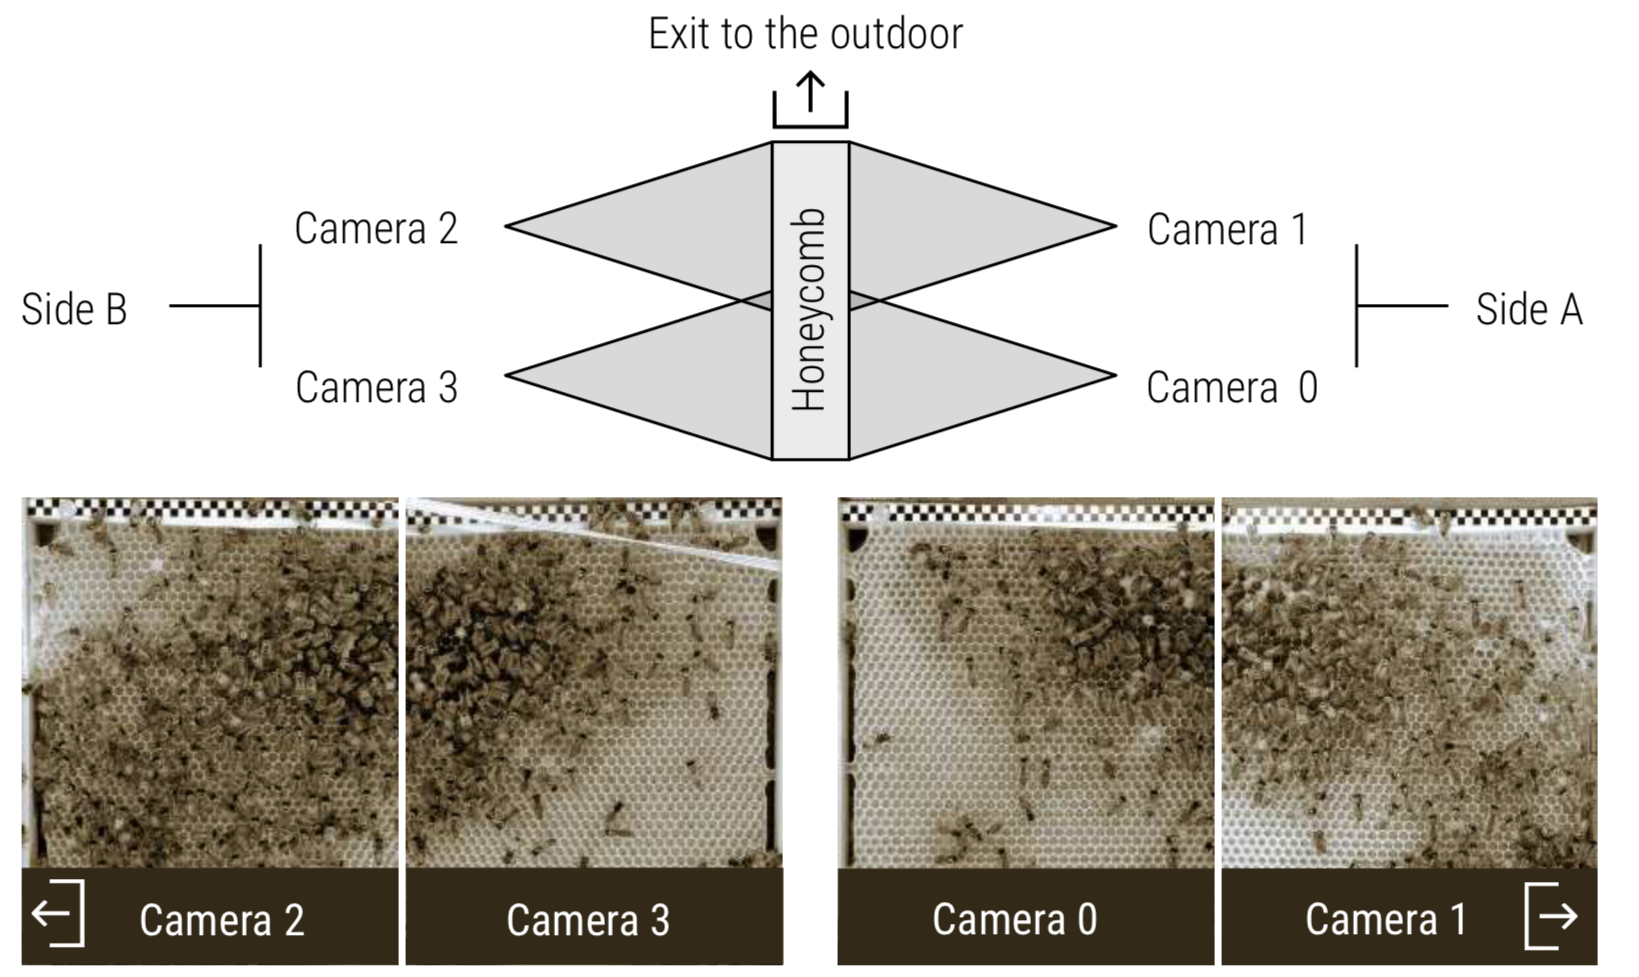
\includegraphics[width=1.0\textwidth]{Chapters/Chapter1/Figs/hive-layout-schlegel.png}
\caption[hive-layout-schlegel]{The observational setup consists of four cameras, with a small field-of-view overlap between the two pairs. The hive exit tube is only accessible from Camera 1 and Camera 2's FOV.
\\(Figure adapted from \cite{schlegel_temporal_2017})}
\label{fig:hive-layout-schlegel}
\end{figure}




The data it collects can be put in 3 categories: 
\begin{itemize}
    \item a list of detections (each assigned to a bee, a point in time and a
    point in the hive space) 
    \item a collection of individuals’ paths (added in [X])
    \item and a collection of bee waggle dance occurrences (added in [X]). 
\end{itemize}
%TODO: are paths separate or integrated: were they added later? what about
%dances?

%TODO: clearpage 


The original \textit{BeesBook} paper put significant focus on waggle dance
research (and providing context around it), but the dataset and collection 
method is meant to serve a very general purpose. 
The system is described to be \textit{“conceived as a budget-priced framework
for the incremental development of software and hardware components”}, capable of
supporting a wide range of investigations into invertebrates, the waggle dance,
honeybee division of labor, collective intelligence and other related fields.



%********************************** %Fourth Section ***************************
\section{This work's goals}
This work’s primary goal is to add building blocks to the \textit{BeesBook}
project by deriving new abstractions that can be used in future analyses and to
show how the process of deriving such abstractions could look like.

A secondary goal is to provide an example of how analysis could be undertaken in
the future, given the data, the set of abstractions and the process for creating
them. 